\section{Markers}
\label{section_markers}

To enable the framework to detect a 3d pose from a video feed, a marker with specific properties will be required.
A marker is a visually significant pattern that the system can detect within an image and can be used to calculate spatial coordinates.
Figure \ref{fig:marker_example} shows an example of such a marker.

Due to our approach for marker detection, we selected a square black on white marker.
Other types exist, such as rotary markers or image-based feature markers.

\begin{figure}
	\centering
	
\includegraphics[width=4cm]{img/marker_example.png}
	\caption[Example Marker.]{An example of a marker. This image is either printed or displayed by some other means in the real world to allow a system to use it as a reference to base a virtual overlay off of it.}
	\label{fig:marker_example}
\end{figure}

\subsection{Coding Scheme}

For this framework, a marker is coded as seen in \ref{fig:marker_template}.
The basis is a 6 by 6 sized grid, where the border is solid black.
The internal 4 by 4 spaces are used to encode the orientation and identification of the marker.
The orientation is encoded by coloring the corners white except for the top right corner, which is encoded black.
The identification is binary encoded with a Hamming code\cite{hamming} for error detection and correction.
Parity bits are the red bits.

\begin{figure}
	\centering
	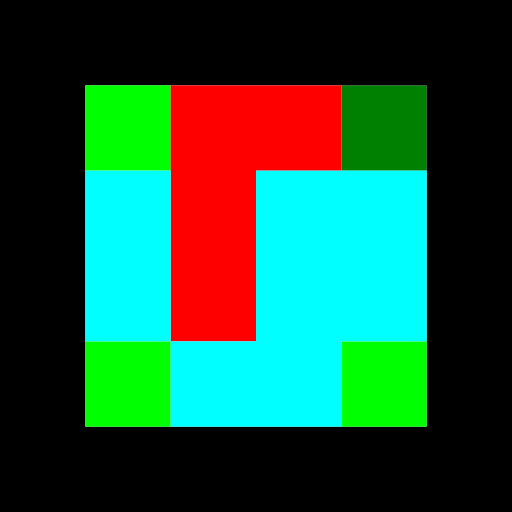
\includegraphics[width=4cm]{img/marker_template.png}
	\caption[Template Marker.]{A color coded representation of a legitimate marker. A real marker is monochrome, the colors here show the location of interesting bits. Green denotes the bits used to determine the rotation: the dark green bit is black, the rest white. Light blue denotes the binary encoded identification number of the marker. Red represents the Hamming encoded parity bits used for error correction.}
	\label{fig:marker_template}
\end{figure}

Thus encoded, the framework can by default detect 256 different markers.
This was deemed sufficient, considering the penalty in performance for each additional detected marker when running on a mobile device, as Imagine becomes unusably slow long before reaching this limit – as seen in section \ref{performance}.

\section{Usage}

For best results when using the markers with our framework, the markers should be printed black on white on a flat surface.
Drawing the markers by hand is possible, but will result in a loss of accuracy due to imperfections that are bound to arise with hand-drawn markers.
Care should especially be taken concerning the outermost border of the marker, as it is the main aspect used for calculating its pose.
Markers that are not smooth or have other imperfections will either outright fail in being identified or have an incorrect pose assigned to them.
